\documentclass[xcolor=pdftex,x11names,table,hyperref]{beamer}

\usepackage{verbatim}
\usepackage{setspace}
\usepackage{amssymb}
\usepackage{url}
\usepackage{xcolor} % See documentation PDF at http://www.ctan.org/pkg/xcolor
\definecolor{darkgreen}{rgb}{0,0.3,0}
\definecolor{darkblue}{rgb}{.05,.05,.30}
\definecolor{lightgrey}{rgb}{0.65,0.65,0.65}
\usepackage{tikzsymbols}


\setbeamertemplate{section in toc}[sections numbered]
\setbeamertemplate{subsection in toc}[subsections numbered]
\setbeamertemplate{subsubsection in toc}[subsubsections numbered]
\usetheme{Singapore}
\setbeamertemplate{navigation symbols}{}
\setbeamertemplate{footline}{%
\vspace{0.0em}%
\hspace{0.5em}%
{\color[rgb]{.1,.1,.1} \insertframenumber{}~/~\inserttotalframenumber}
}

\newcommand{\code}[1]{{\color{darkgreen}\texttt{#1}}}
\newcommand{\detail}[1]{{\color{lightgrey}\small{}#1}}
\newcommand{\teeny}[1]{\scalebox{0.09}{#1}}
\newcommand{\tablecolors}{\rowcolors{2}{blue!12}{white}} % Cool table colors


\begin{document}

\title{Word vectors of various kinds }
\author{\href{http://jon.dehdari.org}{Jon Dehdari} and \textbf{\href{http://www.coli.uni-saarland.de/~asayeed}{Asad Sayeed}}}
\frame{\titlepage}

%\begin{frame}{Good Morning!}
%	\begin{center}
%	%\includegraphics[width=0.8\textwidth]{images/.jpg}
%	\end{center}
%\end{frame}

% what dense word vectors are, pix

\begin{frame}{Jorge Luis Borges}
  An Argentinian philosopher and fiction writer. One of his stories mentions
  'a certain Chinese Encyclopedia', the {\it Celestial Emporium of Benevolent knowledge.} It contains a classifcation of animals.
    \begin{itemize}
    \item those that belong to the emperor
    \item embalmed ones
    \item those that are trained
    \item suckling pigs
    \item mermaids
    \item fabulous ones
    \item stray dogs
    \end{itemize}
\end{frame}

\begin{frame}{Jorge Luis Borges}
  \ldots actually, it goes on.
    \begin{itemize}
    \item those that are included in the present classification
    \item those that tremble as if they are mad
    \item innumerable ones
    \item those drawn with a very fine camelhair brush
    \item others
    \item those that have just broken a flower vase
    \item those that from a long way off look like flies
    \end{itemize}
\end{frame}

\begin{frame}{What words are}
  So far we've talked about words in order.  But words have a
  relationship to each other.
  \begin{itemize}
  \item We use dictionaries in real life for a reason.
  \item We need to make fine-grained distinctions, draw connections,
    and so on.
  \item Humans make judgements about similarities.  
    \begin{itemize}
    \item You know that ``motorcycle'' can be used in most, but not all
      contexts that ``car'' can be used.
    \item English-German bilinguals know that ``pride'' and ``Stolz'' are quite similar.
    \end{itemize}
  \end{itemize}
\end{frame}


\begin{frame}{Define ``chair''}
  From dictionary.com (just the noun version):\pause
  \begin{itemize}
  \item A seat, especially for one person, usually having four legs
    for support and a rest for the back and often having rests for the arms.
  \item Something that serves as a chair or supports like a chair:
    ``two men clasped hands to make a chair for their injured companion''.
  \item A position of authority, as of a judge, professor, etc.
  \item The person occupying a seat of office, especially the chairperson
    of a meeting: ``the speaker addressed the chair''
  \item (in an orchestra) the position of a player, assigned by rank; desk:
    ``first clarinet chair''.
  \item ``the chair'', Informal. electric chair.
  \end{itemize}
\end{frame}

\begin{frame}{Words in terms of other words}
  That doesn't seem very helpful, but it gives us a place to start.\\
  Define ``chair'' in terms of features:
  \begin{itemize}
  \item +one-person, +four-legs, +support, +backrest, +armrest
  \item +authority
  \item +occupies-chair
  \item +orchestra
  \item +execution
  \end{itemize}
\end{frame}

\begin{frame}{Words in terms of other words}
  OK, that gives us the definition of a chair in terms of (rather specific)
  features.\\
  Define the noun ``cockpit". Let's go to dictionary.com again.  I get as features:
  \begin{itemize}
  \item +enclosed, +airplane, +controls, +panel, +seats
  \item +instrumentation, +automobile
  \item +pit, +cockfights
  \item +conflict
  \end{itemize}
  Very little overlaps.
\end{frame}

\begin{frame}{So can we compare them?}
  Encode features as 1 or 0\\
  {\small
  \begin{tabular}{|l|l|l|}
    \hline
    & chair & cockpit \\
    \hline
    one-person & 1 & 0 \\
    backrest & 1 & 0? \\
    four-legs & 1 & 0 \\
    support & 1 & 0? \\
    armrest & 1 & 0? \\
    authority & 1 & 0?\\
    enclosed & 0 & 1\\
    airplane & 0 & 1 \\
    seats & 0? & 1 \\
    \ldots &&\\
    \hline
  \end{tabular}
  }
\end{frame}

\begin{frame}{Similarity}
  \begin{itemize}
  \item What we've just defined is a vector space.\pause
  \item Dimension = feature. So far it's a low-dimensional space.\pause
  \item How can we measure the similarity between them? Common answer:
    cosine similarity.\pause
    %% \begin{block}{Cosine similarity}
    %%   $\mathrm{sim}(\mathbf{A}, \mathbf{B}) = \frac{\mathbf{A} \dot \mathbf{B}}{\norm{\mathbf{A}}\norm{\mathbf{B}}}$
    %% \end{block}\pause
  \item So what would the similarity of ``chair'' and ``cockpit'' be in our space? Probably zero!
  \end{itemize}
\end{frame}

\begin{frame}{Words in terms of other words}
  We need a new data source.  Collect it from a real corpus.  Let's try Google.\\\pause
  {\small
  \begin{tabular}{|l|l|l|}
    \hline
    & chair & cockpit \\
    \hline
    one-person &  &  \\
    backrest &  &  \\
    four-legs &  &  \\
    support &  &  \\
    armrest &  &  \\
    authority &  & \\
    enclosed &  & \\
    airplane & &  \\
    seats &  &  \\
    \ldots &&\\
    \hline
  \end{tabular}
  }\pause\\
  Now it's not so bad: we can get a non-zero similarity.  Yay?
\end{frame}

\begin{frame}{Words in terms of other words}
  \begin{itemize}
  \item In fact, rather than using dictionary definitions of explicit features,
    cut out the middle man.\pause
  \item ``Learn'' a vector for each word by counting corpus context. Ways of learning:
    \begin{itemize}
    \item Simple co-occurrence counts based on a window.
      \begin{itemize}
      \item The vocabulary basically becomes the feature space.
      \end{itemize}\pause
    \item More complex counts, such as POS tags, bits of parse trees.\pause
    \end{itemize}
  \item Sometimes raw counts aren't what you need: smoothing, reweighting.
  \end{itemize}
\end{frame}

\begin{frame}{Words in terms of other words}
  These are ``count'' vectors. 
  What are the problems with doing it this way?\pause
  \begin{itemize}
    \item Sparsity: many words just never appear with other words.\pause
    \item Dimensionality: especially if you use fancy features (syntax, etc),
      you get million dimensional spaces.\pause
  \end{itemize}
  What we need? Dimensionality reduction, or some other way to start
  from a compressed space.\pause
  \begin{itemize}
  \item Sharing dimensions helps generalization.\pause
  \item Nevertheless, there's value in count vectors (for things that require explicit linguistic knowledge)\pause
  \end{itemize}
  So now\ldots ``predict'' vectors\ldots
\end{frame}

\begin{frame}{Words as Integers}
\begin{itemize}
	\item Our previous representations of words (and word classes) have been fairly flat
	\item For example, the word `\textit{monkey}' can be represented as an integer, such as `7'
	\pause
	\item \textbf{One-hot encoding} represents that as: \\[0.4em]
		\begin{tabular}{|c|c|c|c|c|c|c|c|c|c|c|c|}
		    \hline
			%\colorbox{black}{\color{white}1}
			0 & 0 & 0 & 0 & 0 & 0 & 1 & 0 & 0 & 0 & \ldots & 0 \\
		    \hline
		\end{tabular}
	\pause

\item and the word class (eg.\ 2) containing `\textit{monkey}': \\[0.4em]
		\begin{tabular}{|c|c|c|c|}
		    \hline
			0 & 1 & 0 & 0 \\
		    \hline
		\end{tabular}

	\pause
	\item Both of these are sparse vectors of booleans, with just one entry having a `true' value
	\pause
	\item Either way, we're working with integers {\small (\ldots, -2, -1, 0, 1, 2, \ldots)}
\end{itemize}
\end{frame}


\begin{frame}{\includegraphics[width=0.06\textheight]{images/real_madrid_cf.png} \hspace{1.5em} Words as $\mathbb{R}$eal Numbers}
\begin{itemize}
	\item We can do more with real numbers (eg. -1.5, 0.23, 55.01)
	\pause
	\item We can represent the word `\textit{monkey}' as a dense vector of real numbers: \\[0.4em]
		\begin{tabular}{|c|c|c|c|}
		    \hline
			0.38 & -1.27 & -0.55 & 1.44 \\
		    \hline
		\end{tabular}
	\pause
	\item We can have the plural form, `\textit{monkeys}' be close in that vector space: \\[0.4em]
		\begin{tabular}{|c|c|c|c|}
		    \hline
			\bf 0.31 & -1.27 & \bf -0.61 & 1.44 \\
		    \hline
		\end{tabular}
	\pause
	\item We can also have a related word, like `\textit{ape}' be close in that vector space, \emph{but in different dimensions}: \\[0.4em]
		\begin{tabular}{|c|c|c|c|}
		    \hline
			0.38 & \bf -1.33 & -0.55 & \bf 1.49 \\
		    \hline
		\end{tabular}
\end{itemize}
\end{frame}


% applications: analogy, qa, nnlm's
\begin{frame}{Applications of Word Vectors}
\begin{itemize}
	\item \textbf{Word distances}.  For example, closest words to `\textit{Sweden}':
		\begin{center}
		\begin{footnotesize}
		\begin{tabular}{rl}
			\bf Word & \bf Cosine Distance \\
			\hline
			Norway & 0.75 \\
			Denmark & 0.72 \\
			Finland & 0.62 \\
			Switzerland & 0.59 \\
			\ldots & \\
		\end{tabular}
		\end{footnotesize}
		\end{center}
		\pause
	\item \textbf{Analogy}.  E.g., \textit{Japan} is to \textit{Tokyo} as \textit{Germany} is to \textit{Berlin}
		\begin{center}
		\includegraphics[width=0.54\textwidth]{images/countries_capitals.png}
		\end{center}
		\pause
		{\scriptsize Japan -- Tokyo $\approx$ Germany -- Berlin }
\end{itemize}
\end{frame}


\begin{frame}{Applications of Word Vectors}
\begin{itemize}
	\item \textbf{\href{http://research.microsoft.com/en-us/um/people/cburges/tech_reports/msr-tr-2011-129.pdf}{Sentence Completion}} (actually just restricted language modeling):
	\item ``All red-headed men who are above the age of {\color{darkblue} [ 800 $|$ seven $|$ twenty-one $|$ 1,200 $|$ 60,000 ]} years , are eligible.''
	\item ``That is his {\color{darkblue} [ generous $|$ mother's $|$ successful $|$ favorite $|$ main~]} fault , but on the whole he's a good worker.''
	\pause
	\item \href{http://arxiv.org/pdf/1301.3781.pdf}{Mikolov et al (2013b)} selected the test word that best predicted the context
\end{itemize}
\end{frame}


% models, relationship with projection layers of nnlm's
\begin{frame}{Projection Layer in Neural Language Models}
\begin{itemize}
	\item \textbf{Neural Language Modeling} -- this was actually one of the earliest uses of word vectors.  We'll talk more about these later this semester \\
		\begin{center}
		\includegraphics[width=0.55\textwidth]{images/bengio-etal2003_pg6_image_alt.pdf}
		\end{center}
\end{itemize}
\end{frame}


% word2vec: cbow, sg
\begin{frame}{word2vec}
\begin{itemize}
	\item Tom\'{a}\v{s} Mikolov and colleagues found that you don't need the full neural-net language model to get useful word vectors
	\pause
	\item In fact, you don't need a neural network at all. He removed the hidden layer, giving a traditional log-linear model
	\pause
	\item He developed a simplified form of training called negative sampling (derived from earlier NCE).  It's a little like a binary MaxEnt classifier
\end{itemize}
\end{frame}


\begin{frame}{word2vec: CBOW \& Skip-gram}
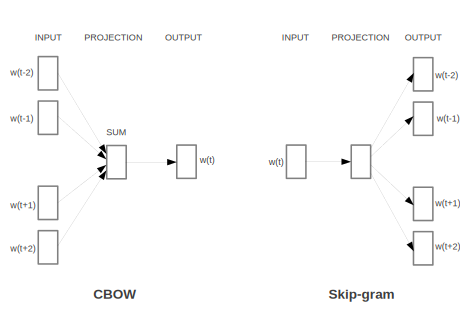
\includegraphics[width=0.90\textwidth]{images/mikolov-etal2013b_fig1.png}
%\begin{itemize}
%	\item 
%	\item 
%\end{itemize}
\end{frame}


\begin{frame}{Hyperparameters}
\begin{itemize}
	\item Window size: how much surrounding context to use
	\item Normalization: softmax (traditional) vs.\ hierarchical softmax vs.\ negative sampling
	\item Vector dimensions: 100--500 common
	\item Number of negative samples: 3--10 common
	\item Number of training epochs, initial learning rate, negative sample distribution ($\alpha = 0.75$), model, \ldots
\end{itemize}
\end{frame}




\begin{frame}{Matrix Factorization of Count Co-Occurrences}
\begin{itemize}
	\item Glove and Latent Semantic Analysis (LSA) count the co-occurrences of word pairs, then use matrix factorization techniques like singular value decomposition (SVD) for dimensionality reduction of this original matrix \\
		\begin{center}
		\includegraphics[width=0.42\textwidth]{images/singular-value-decomposition_from_wp.png}
		\end{center}
\end{itemize}
\end{frame}

\begin{frame}{Unifying these Approaches}
\begin{itemize}
	\item Word2vec, Glove, and LSA all do matrix factorization \href{https://levyomer.files.wordpress.com/2014/09/neural-word-embeddings-as-implicit-matrix-factorization.pdf}{(Levy \& Goldberg, 2014)}, but the successful ones are weighted for word frequency
	\item Pointwise Mutual Information (PMI) is (implicitly) used by these:
		\begin{equation*}
			\text{PMI}(x,y) = log \frac{P(x,y)}{P(x) \, P(y)}
		\end{equation*}
\end{itemize}
\end{frame}


\begin{frame}{Bilingual Word Vectors}
\begin{center}
	\includegraphics[height=0.42\textheight]{images/hermann-blunsom2013_fig3.pdf}
\end{center}

\pause
Monolingual objective: maximize likelihood of training set, where $P(w|c) = \sigma({\bf w \cdot c})$ \\[1.0em]
Multilingual objective: maximize likelihood of both sentence-aligned training sets (s \& t), based on: $\sigma({\bf w_t \cdot c_t}) + \sigma({\bf w_t \cdot c_s}) + \sigma({\bf w_s \cdot c_s}) + \sigma({\bf w_s \cdot c_t})$

\vspace*{2.0em}
{\tiny Courtesy of \href{http://arxiv.org/abs/1312.6173}{Hermann \& Blunsom (2013)}}
\end{frame}


\begin{frame}{Bilingual Word Vectors Comparison}
\vspace*{4.0em}%
\begin{spacing}{1.2}
\begin{scriptsize}
\hspace*{-2.5em}%
\begin{tabular}{l|llllll}
	Method & \parbox[c]{4.5em}{No word alignments required} & \parbox[c]{4.4em}{No prior on the mapping between target vectors} & \parbox[c]{4.5em}{No explicit alignments of target vectors} & \parbox[c]{3.9em}{Compu\-tation\-ally efficient} & \parbox[c]{3.5em}{Can leverage monolingual corpus} & \parbox[c]{3.6em}{Free software} \\[0.7em]
	\hline
	{\tiny \href{https://www.aclweb.org/anthology/C12-1089.pdf}{Klementiev et al (2012)}} & \checkmark & x & \checkmark & x & \checkmark & x \\
	%  (Hermann \& Blunsom, 2013)
	\href{http://arxiv.org/abs/1312.6173}{BiCVM} & \checkmark & \checkmark & x & \checkmark & x & \color{blue}{\href{https://github.com/karlmoritz/bicvm}{\checkmark}} \\
	%  (Chandar et al, 2014)
	{\tiny \href{http://papers.nips.cc/paper/5270-an-autoencoder-approach-to-learning-bilingual-word-representations}{Bilingual autoencoders}} & \checkmark & \checkmark & x & x & x & \color{blue}{\href{http://sarathchandar.in/data/corr_net.zip}{\checkmark}} \\
	% (Gouws et al, 2014) 
	\href{http://arxiv.org/abs/1410.2455}{BilBOWA} & \checkmark & \checkmark & x & \checkmark & \checkmark & \color{blue}{\href{https://github.com/gouwsmeister/bilbowa}{\checkmark}}  \\
	% (Coulmance et al, 2015)
	\href{https://www.aclweb.org/anthology/D15-1131.pdf}{Trans-gram} & \checkmark & \checkmark & \checkmark & \checkmark & \checkmark & x \\
\end{tabular} \\[7.0em]
\end{scriptsize}
\end{spacing}
{\tiny Courtesy of \href{https://www.aclweb.org/anthology/D15-1131.pdf}{Coulmance et al.\ (2015)}}
\end{frame}


\begin{frame}{Try Them Out!}
\begin{itemize}
	\item Original word2vec code: \url{https://code.google.com/p/word2vec/} -- includes nice illustrations
	\item Python version: \href{http://radimrehurek.com/gensim}{Gensim}
	\item Java version in \href{http://deeplearning4j.org/word2vec.html}{DL4J}
	\item \href{http://nlp.stanford.edu/projects/glove}{Glove}
\end{itemize}
\end{frame}





% \begin{frame}{}
% \begin{block}{}
% \begin{itemize}
% 	\item 
% 	\item 
% 	\item 
% \end{itemize}
% \end{block}
% \end{frame}


\end{document}
